\subsection*{\center Ejercicio 5C. Teoría del consumidor}
\vspace{1cm}

\subsubsection*{\center I. Describiendo los gustos individuales.}
\vspace{.5cm}

Invita a unos amigos a ver un partido en casa. Sus amigos quieren patatas fritas y cervezas, por lo que acude al supermercado donde existen dos tipos de mercancías: $‘$bolsas de patatas fritas$’$ (mercancía $1$) y $‘$latas de cerveza sueltas$’$ (mercancía $2$) (es decir, en el eje de abcisas vamos a indicar las patatillas y el de ordenadas las cervezas sueltas). En concreto, los gustos de sus amigos son tomar una bolsa de patatillas fritas por cada dos cervezas.\\\\

\begin{enumerate}[\Large \bfseries 1.]

    %----------1.
    \item \textbf{¿Qué relación binaria caracteriza sus gustos con respecto a estas dos mercancías?}\\\\
	\textbf{Respuesta.-}\; En primer lugar el conjunto de consumo viene dado por las patatas fritas y las cervezas, es decir, $$\mathcal{X}^i = \lbrace x \in \mathbb{Z}^2 \; : \; x_l \geq 0 \; \mbox{para} \; l=1,2\rbrace.$$
	En segundo lugar, identificamos las cestas indiferentes. Por ejemplo, la cesta $"$bolsas de patatas fritas$"$ $\left( \mbox{cesta}\; (1,0) \right)$, es indiferente a la cesta $"$latas de cervezas sueltas$"$ $\left(\mbox{cesta}\; (0,2) \right)$, ya que, 
    $$\left.\begin{array}{rcl} (1,0)&\succeq&(0,2) \\ (0,2) & \succeq&(1,0) \end{array}\right\}\Longrightarrow (1,0) \sim (2,0)$$\\
	\begin{center}
	    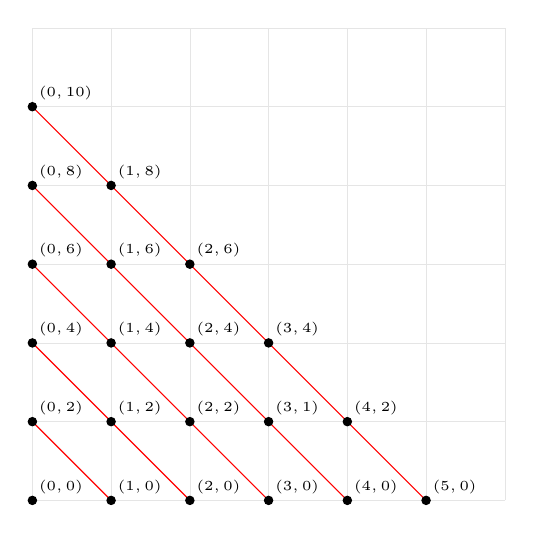
\begin{tikzpicture}
		% abscisa y ordenada
		\tkzInit[xmax= 5.5,xmin=0,ymax=11,ymin=0,ystep=2]
		\tiny\tkzLabelX[opacity=0.4,step=1, orig=false]
		\tiny\tkzLabelY[opacity=0.4,step=1, orig=false]
		% label x, f(x)
		\tkzDrawX[opacity= 1,label=Patatas fritas , right=.5]
		\tkzDrawY[opacity= 1,label=Latas de cervezas, below = -.5]
		%dominio y función
		\draw[step=1cm,black,very thin,opacity=.1] (0,0) grid (6,6);
		\draw[color=red](1,0)--(0,1);
		\draw[color=red](2,0)--(0,2);
		\draw[color=red](3,0)--(0,3);
		\draw[color=red](4,0)--(0,4);
		\draw[color=red](5,0)--(0,5);

		\filldraw[black] (0,0)node[above right]{$(0,0)$} circle (1.5pt);

		\filldraw[black] (1,0)node[above right]{$(1,0)$} circle (1.5pt);
		\filldraw[black] (0,1)node[above right]{$(0,2)$} circle (1.5pt);

		\filldraw[black] (2,0)node[above right]{$(2,0)$} circle (1.5pt);
		\filldraw[black] (1,1)node[above right]{$(1,2)$} circle (1.5pt);
		\filldraw[black] (0,2)node[above right]{$(0,4)$} circle (1.5pt);

		\filldraw[black] (3,0)node[above right]{$(3,0)$} circle (1.5pt);
		\filldraw[black] (2,1)node[above right]{$(2,2)$} circle (1.5pt);
		\filldraw[black] (1,2)node[above right]{$(1,4)$} circle (1.5pt);
		\filldraw[black] (0,3)node[above right]{$(0,6)$} circle (1.5pt);

		\filldraw[black] (4,0)node[above right]{$(4,0)$} circle (1.5pt);
		\filldraw[black] (3,1)node[above right]{$(3,1)$} circle (1.5pt);
		\filldraw[black] (2,2)node[above right]{$(2,4)$} circle (1.5pt);
		\filldraw[black] (1,3)node[above right]{$(1,6)$} circle (1.5pt);
		\filldraw[black] (0,4)node[above right]{$(0,8)$} circle (1.5pt);

		\filldraw[black] (5,0)node[above right]{$(5,0)$} circle (1.5pt);
		\filldraw[black] (4,1)node[above right]{$(4,2)$} circle (1.5pt);
		\filldraw[black] (3,2)node[above right]{$(3,4)$} circle (1.5pt);
		\filldraw[black] (2,3)node[above right]{$(2,6)$} circle (1.5pt);
		\filldraw[black] (1,4)node[above right]{$(1,8)$} circle (1.5pt);
		\filldraw[black] (0,5)node[above right]{$(0,10)$} circle (1.5pt);
	    \end{tikzpicture}
	\end{center}
	\vspace{.5cm}

	Análogamente la cesta $(2,0)$ es indiferente a las cestas $(0,4)$ y $(1,2)$, como también la cesta $(3,0)$ es indiferente a las cestas $(0,6),\; (1,4)$ y $(2,2)$. Por lo tanto una cesta $x=(x_1,x_2)$ es indiferente a otra $y=(y_1,y_2)$ si, $$2x_1 + x_2 = 2y_1 + y_2.$$
	Por último caracterizamos formalmente los gustos a través de la relación binaria $"$ser como mínimo tan preferido como$"$ como sigue,
	\begin{center}
	    Dado cualquier par de cestas $x,y \in \mathcal{X}^i$ entonces $x \succeq^i y \; \Longleftrightarrow 2x_1 + x_2 \geq 2y_1 + y_2$.
	\end{center}
	\vspace{.5cm}

    %----------2.
    \item \textbf{¿Puede representar sus gustos a través de conjuntos de indiferencia?}\\\\
	\textbf{Respuesta.-} Si podemos. Siendo que cumplen los axiomas de completitud y transitividad, tenemos que,
	$$x,y\in \mathcal{X}^i \; \mbox{entonces} \; x\succeq^i y \; \Longleftrightarrow \; 2x_1+x_2 \geq 2y_1+y_2.$$
	Luego y sabiendo que las ordenaciones serán consistente, es decir, que podemos identificar conjuntos de cestas indiferentes, podemos definirlas como, 
	$$\mathcal{I}^i(x) = \lbrace y\in \mathcal{X}^i\; : \;  2x_1 + x_2 = 2y_1 + y_2\rbrace.$$
	Y por lo tanto, los gustos están representados por $\left(\mathcal{X}^i,\lbrace \mathcal{I}^i(x)\rbrace_{x\in \mathcal{X}^i}\right)$. Por ejemplo, ya que $2\cdot 1 + 0 = 2\cdot 0 + 2$ entonces,
	$$\mathcal{I}^i (1,0) = \lbrace (0,2) \rbrace$$
	
	\begin{center}
	    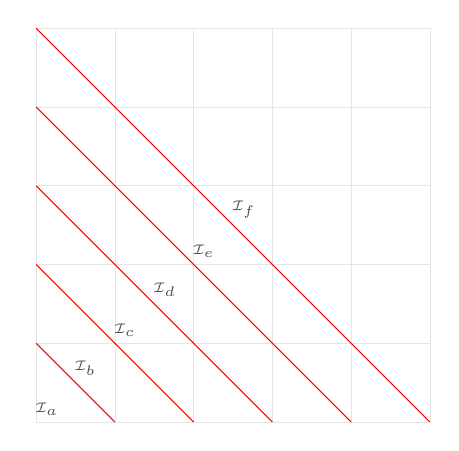
\begin{tikzpicture}
		% abscisa y ordenada
		\tkzInit[xmax= 5,xmin=0,ymax=10,ymin=0,ystep=2]
		\tiny\tkzLabelX[opacity=0.4,step=1, orig=false]
		\tiny\tkzLabelY[opacity=0.4,step=1, orig=false]
		% label x, f(x)
		\tkzDrawX[opacity= 1,label=Patatas fritas , right=.5]
		\tkzDrawY[opacity= 1,label=Latas de cervezas, below = -.5]
		%dominio y función
		\draw[step=1cm,black,very thin,opacity=.1] (0,0) grid (5,5);
		\draw[color=red](1,0)--(0,1);
		\draw[color=red](2,0)--(0,2);
		\draw[color=red](3,0)--(0,3);
		\draw[color=red](4,0)--(0,4);
		\draw[color=red](5,0)--(0,5);
		\draw[opacity=.7](-.1,0)node[above right]{$\mathcal{I}_a$};
		\draw[opacity=.7](.4,.5)node[above right]{$\mathcal{I}_b$};
		\draw[opacity=.7](.9,1)node[above right]{$\mathcal{I}_c$};
		\draw[opacity=.7](1.4,1.5)node[above right]{$\mathcal{I}_d$};
		\draw[opacity=.7](1.9,2)node[above right]{$\mathcal{I}_e$};
		\draw[opacity=.7](2.4,2.5)node[above right]{$\mathcal{I}_f$};
	    \end{tikzpicture}
	\end{center}
	\vspace{.5cm}
	De manera similar $$\mathcal{I}^i(2,0) = \lbrace (1,2),(0,4) \rbrace \quad;\quad \mathcal{I}^i(3,0) = \lbrace (2,2),(1,4),(0,6) \rbrace$$\\

    %----------3.
    \item \textbf{¿Puede representar sus gustos a través de una función de utilidad?}\\\\


\subsubsection*{\center II. Elección óptima.}
\vspace{.5cm}

\subsubsection*{\center III. Curva de demanda.}
\vspace{.5cm}

\subsubsection*{\center IV. Cálculo analítico de la fu:nción de demanda.}
\vspace{.5cm}

\end{enumerate}
